\section{Couplage conduction-rayonnement dans TRUST}


Les chapitres précédents ont permis de vérifier le calcul des facteurs de vue ainsi que le calcul des échanges radiatifs entre surfaces diffuses grises. L'objectif est désormais d'intégrer ce modèle au sein d'un code de calcul thermique afin de simuler le couplage entre la conduction dans les solides et les échanges radiatifs en milieu transparent.

La plateforme \textsc{TRUST} (\textit{TRio\_U Software for Thermal-hydraulics}) \footnote{\url{(https://cea-trust-platform.github.io/}}\cite{saikali2025trust}, développée par le CEA, est un environnement de simulation multiphysique reposant sur une discrétisation par volumes finis. Initialement conçue pour la thermohydraulique, elle permet également de résoudre des problèmes de conduction thermique, de convection et de transferts couplés sur des géométries complexes. Son architecture modulaire facilite l'ajout de nouveaux modèles physiques, ce qui en fait un support adapté au développement d'un modèle de rayonnement thermique en milieu transparent.

Des travaux préliminaires ont été réalisés au CEA autour du couplage conduction-rayonnement à l'aide de la maquette \texttt{python} \texttt{pyMCRAD}, développée par Romain Le Tellier. Cette maquette a permis de démontrer la faisabilité du couplage entre le calcul des facteurs de vue et la résolution thermique. En revanche, elle repose sur des facteurs de vue préalablement connus et reste limitée à des géométries bidimensionnelles simples. L'objectif du présent travail est de lever ces limitations en intégrant directement le calcul des facteurs de vue à partir du maillage utilisé par \textsc{TRUST}, afin de permettre la simulation de géométries tridimensionnelles quelconques.




\section{Problème physique étudié}

Le domaine étudié est constitué de plusieurs solides séparés par un milieu transparent, comme illustré Figure~\ref{fig:domaine}. Les échanges thermiques dans les solides sont gouvernés par la conduction, tandis que les surfaces en contact avec le milieu transparent échangent de l'énergie par rayonnement. Le milieu transparent n'absorbe ni n'émet de rayonnement ; il constitue uniquement le support de propagation des rayons entre les surfaces.

\begin{figure}[H]

\begin{minipage}{0.55\textwidth}
    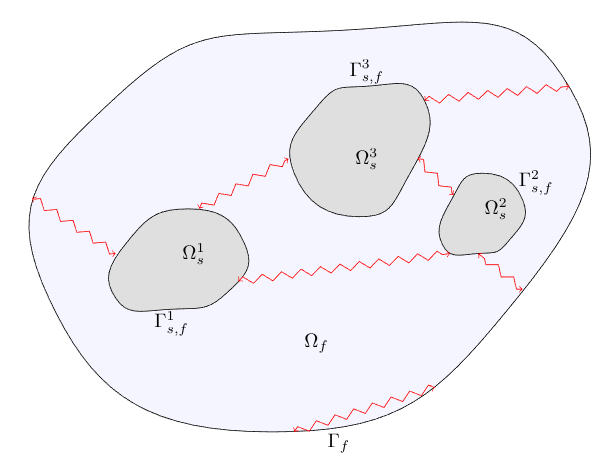
\includegraphics[width=1\linewidth]{PICTURES/domaine.png}
    

    
\end{minipage}
\hfill
\begin{minipage}{0.4\linewidth}
    Notations :
    
    $\Omega_s^i$ les différents domaines solides.
    
    $\Omega_s$ le domaine fluide.
    
    $\Gamma^i_{s,f}$ l'interface entre le solide $i$ et le fluide.
    
    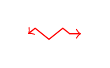
\begin{tikzpicture} 
        \draw[<->, red , decorate, decoration={zigzag, amplitude=2pt}]
        (0, 0) -- (0.67,0);
    \end{tikzpicture} Un symbole pour le couplage.
\end{minipage}
\caption{Schéma typique d’un problème de couplage conduction-rayonnement en milieu transparent}
\label{fig:domaine}
\end{figure}

Dans chaque domaine solide $\Omega_s^i$, la température est obtenue par résolution de l'équation de la chaleur

\begin{equation}
\rho_s^i C_p^i
\frac{\partial T}{\partial t}
=
\nabla\cdot
\left(
\lambda_s^i
\nabla T
\right)
+
\dot q_{\mathrm{vol}}.
\end{equation}

Dans cette étude, le milieu transparent n'intervient pas directement dans le transport radiatif. Lorsque sa résolution thermique est nécessaire, sa température est obtenue à partir de l'équation classique de diffusion

\begin{equation}
\rho_f C_{p,f}
\frac{\partial T}{\partial t}
=
\nabla\cdot
\left(
\lambda_f
\nabla T
\right)
+
\dot q_{\mathrm{vol}}.
\end{equation}

Le couplage entre les domaines solides et le milieu transparent est assuré aux interfaces $\Gamma_{s,f}^i$. La température est supposée continue et le bilan des flux s'écrit

\begin{equation}
\left\{
\begin{aligned}
T_s &= T_f,\\
-\lambda_s\nabla T_s\cdot\mathbf n
&=
-\lambda_f\nabla T_f\cdot\mathbf n
+
q_r,
\end{aligned}
\right.
\end{equation}

où $q_r$ désigne le flux radiatif net calculé à partir des facteurs de vue présentés au chapitre précédent.

Dans le cadre de ce stage, l'étude se limite au couplage entre la conduction dans les solides et les échanges radiatifs de surface à surface. Les simulations sont réalisées sous les hypothèses de surfaces opaques, diffuses grises, d'un milieu transparent et de propriétés thermophysiques constantes.

	
	
	\section{Cas de vérification sur une géométrie bidimensionnelle infinie}

Afin de vérifier le couplage entre le solveur thermique \trust et le module de calcul radiatif développé au cours de ce stage, les résultats obtenus sont comparés à ceux de la maquette de référence \texttt{pyMCRAD}. Cette dernière constitue un cas de validation pertinent puisqu'elle implémente le même modèle physique de conduction-rayonnement en milieu transparent pour des géométries bidimensionnelles.

Le cas considéré représente une rangée infinie de crayons combustibles modélisée par un motif élémentaire de dix crayons. Les conditions de périodicité suivant la direction verticale permettent de reproduire un milieu infini, le motif étant illustré à la Figure~\ref{fig:domaine}. Les facteurs de vue sont cette fois calculés directement à partir du maillage par le module MCRT, puis utilisés dans la résolution thermique sous \trust.

\begin{figure}[H]

\begin{minipage}{0.2\textwidth}
    \centering
    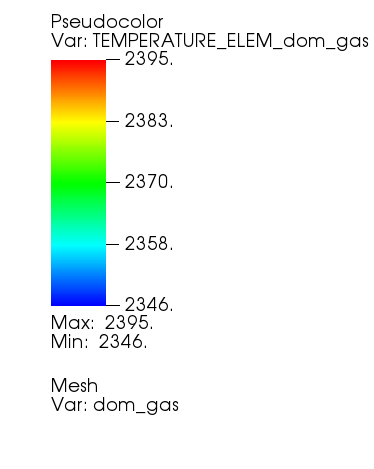
\includegraphics[width=\linewidth]{PICTURES/c5couplage/legend.png}
\end{minipage}
\hfill
\begin{minipage}{0.75\linewidth}
    \centering
    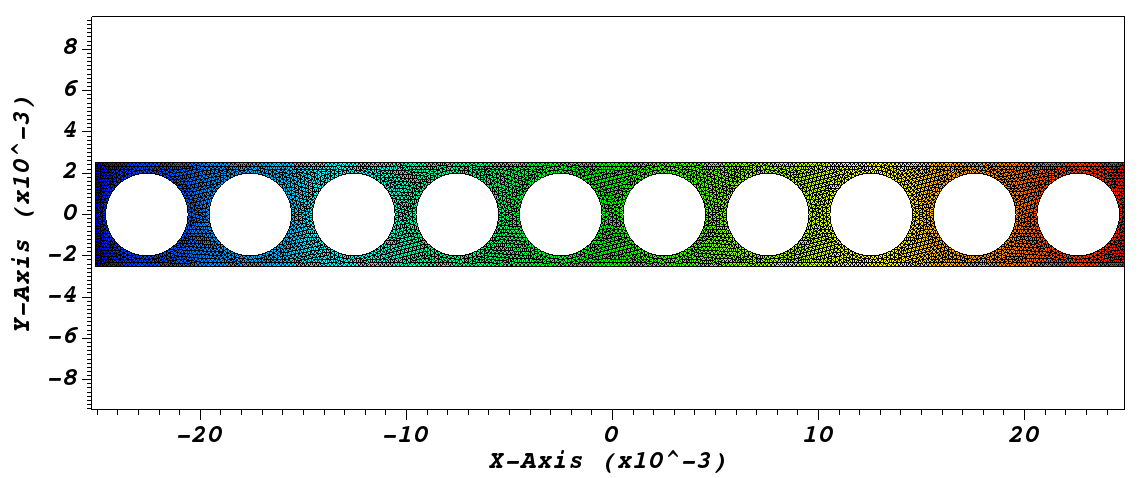
\includegraphics[width=\linewidth]{PICTURES/c5couplage/mesh.png}
\end{minipage}

\caption{Motif élémentaire de dix crayons répété périodiquement suivant les directions $y^+$ et $y^-$.}
\label{fig:domaine}

\end{figure}

La comparaison est réalisée au travers de la conductivité thermique équivalente apparente $K_a$, grandeur classiquement utilisée pour caractériser les transferts thermiques dans les milieux poreux \cite{romain26}. Celle-ci est définie par

\begin{equation}
K_a(T_0)=
\frac{R}{2L_Y\Delta T}
\int_{\Gamma_L\cup\Gamma_R}
\left|\mathbf q\cdot\mathbf n\right|
\,\mathrm dS,
\end{equation}

où $\mathbf q$ désigne le flux thermique total traversant les frontières latérales du domaine.

\begin{figure}[H]
\centering
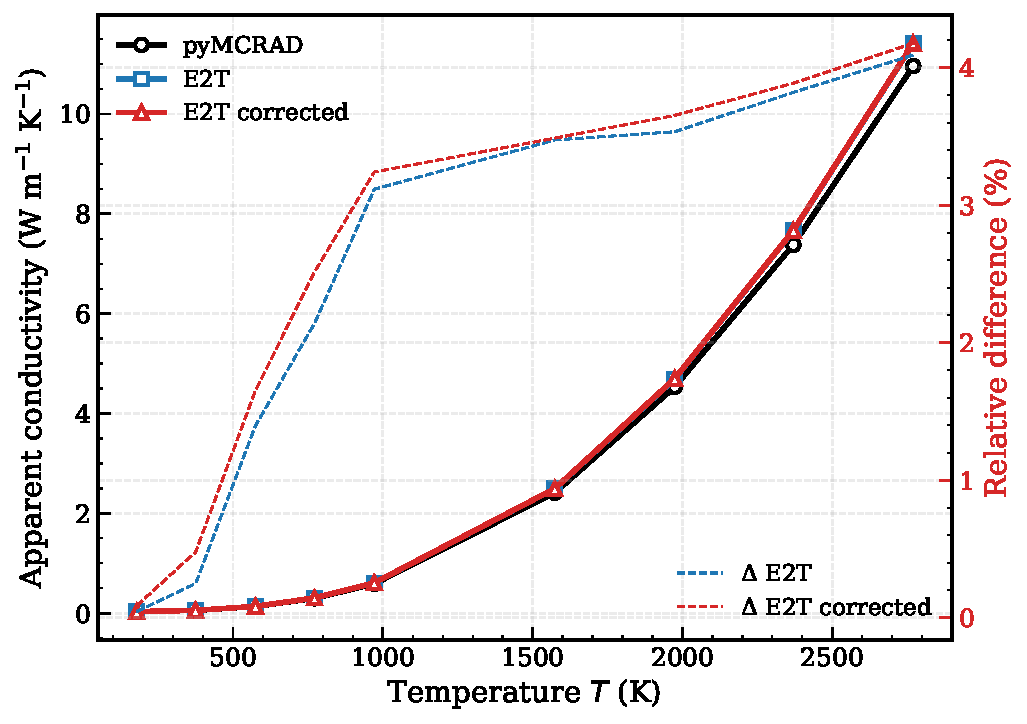
\includegraphics[width=0.9\linewidth]{PICTURES/c5couplage/Ka_vs_T.pdf}
\caption{Comparaison de la conductivité thermique équivalente obtenue avec \textsc{TRUST} et \texttt{pyMCRAD}.}
\label{fig:ka}
\end{figure}

La Figure~\ref{fig:ka} met en évidence un bon accord entre les deux approches sur l'ensemble de la plage de températures étudiée. Les deux modèles reproduisent la même évolution de la conductivité équivalente lorsque la température augmente, ce qui confirme la bonne intégration du calcul radiatif au sein de \textsc{TRUST}.

Les écarts les plus importants apparaissent aux températures les plus élevées. Ce comportement est attendu puisque la contribution du rayonnement devient alors prépondérante, les échanges radiatifs évoluant comme la quatrième puissance de la température. Dans ces conditions, une faible variation des facteurs de vue se traduit directement par une variation plus importante des flux radiatifs.

L'écart maximal observé reste inférieur à 5~\%. Il est principalement attribué aux différences de représentation géométrique entre les deux modèles. Dans le cas présent, les crayons combustibles sont discrétisés par des polygones réguliers de 64 côtés. Comme discuté en Annexe~\ref{annexe:geom}, cette approximation modifie légèrement les facteurs de vue géométriques. Or, l'étude de sensibilité présentée en Section~\ref{part:hypersens} a montré que les flux radiatifs sont particulièrement sensibles à de faibles variations des facteurs de vue. Les écarts observés restent néanmoins compatibles avec cette approximation géométrique et valident le couplage conduction-rayonnement développé dans \textsc{TRUST}.


